\documentclass[12pt]{article}
\usepackage[utf8]{inputenc}
\usepackage{polski}
\usepackage{enumitem}
\usepackage{amsmath}
\usepackage{tikz}

\title{Zadanie 2--4}
\author{Patryk Lisik}
\date{\(15\) Grudnia  2023}

\begin{document}

\maketitle
\renewcommand{\abstractname}{Treść}

\begin{abstract}
    Znajdź prawdopodobieństwa warunkowe $\text{Pr}(X=x_i|Y=y_j)$ dla binarnego kanału wymazującego
    o prawdopodobieństwie wymazania $\text{Pr}(Y=?|X= 0) = \text{Pr}(Y=?|X= 1) = 0.469$,
    jeżeli prawdopodobieństwa nadania wiadomości ze źródła są $\text{Pr}(X= 0) = 0.25$  i $\text{Pr}(X= 1) = 0.75$.
    Znajdź ekwiwokację, informację wzajemną i pojemność kanału.
\end{abstract}


\section*{Rozwiązanie}

Prawdopodobieństwa warunkowe:
\begin{align*}
    & \text{Pr}(X=0|Y=0) = &0.531 \cdot 0.25 =& 0.13275\\  
    & \text{Pr}(X=0|Y=1)  & = & 0.0 \\
    & \text{Pr}(X=0|Y=?) = &0.469 \cdot 0.25 =& 0.11725 \\
    & \text{Pr}(X=1|Y=0)  & = & 0.0 \\
    & \text{Pr}(X=1|Y=1) = &0.531 \cdot 0.75 = & 0.39825 \\
    & \text{Pr}(X=1|Y=?) = &0.469 \cdot 0.75 = & 0.35175
\end{align*}

Ekwiwokacja:
\begin{align*}
    & q_0 = \text{Pr}(X=0|Y=0) \\
    & q_1 = \text{Pr}(X=1|Y=1) \\
    & q_? = \text{Pr}(X=0|Y=?) + \text{Pr}(X=1|Y=?) = 0.469 \\
    & H(X|Y) = \sum_j q_j H(X,y_j) 
     = q_0H(X,y_0) + q_1H(X,y_1) + q_1H(X,y_?) =  \\
    & = q_0\left( - \text{Pr}(X=0|Y=0)\log_2\text{Pr}(X=0|Y=0)  +  \text{Pr}(X=0|Y=1)\log_2\text{Pr}(X=0|Y=1) \right) + \\ 
    & + q_1 \left( - \text{Pr}(X=1|Y=1)\log_2\text{Pr}(X=1|Y=1) + \text{Pr}(X=1|Y=0)\log_2\text{Pr}(X=1|Y=0)\right) + \\
    & + q_? \left( - \text{Pr}(X=0|Y=?)\log_2\text{ Pr}(X=0|Y=?) -
                     \text{Pr}(X=1|Y=?)\log_2\text{ Pr}(X=1|Y=?) \right) \\
    & = 0.13275 \cdot ( - 0.13275 \cdot \log_2 0.13275  + 0) + 0.39825 \cdot (- 0.39825 \cdot \log_2 0.39825 + 0) \\
    & + 0.469 \cdot ( - 0.11725 \cdot \log_2 0.11725 - 0.35175 \cdot \log_2 0.35175 ) \\
    & = 0.051 + 0.211 + 0.419 =  0.681
\end{align*}

Dlaczego $0 \cdot \log_2 =0 $?

$$ 
\lim_{x\to 0^+} x \log x=\frac{\log x}{x^{-1}}  \overset{\mathrm{H}}{=} \frac{\frac{1}{x}}{x^{-2}}=x = 0
$$

W tym działaniu wyobrażamy sobie $x\log x$ jako funkcję 
$$ 
x\log x = 
\begin{cases}
    x\log x &  \text{dla }   x \ne 0 \\
    0      &  \text{dla }   x = 0
\end{cases}
$$

Informacja wzajemna: 
\begin{align*}
    & I(X;Y) = H(X) - H(X|Y) \\
    & H(X) =- \sum_i p_i \log_2 p_i = -0.25\cdot \log_2 0.25 - 0.75 \cdot \log_2 0.75 = 0.811 \\
    & I(X;Y) = 0.811 - 0.681 = 0.13
\end{align*}

Pojemność kanału:

\begin{figure}[h]
    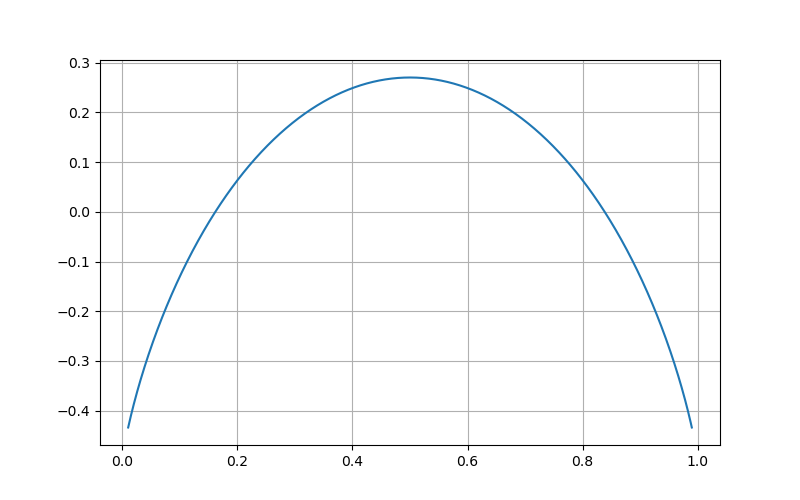
\includegraphics[width=14cm]{infromacja_wzajemna.png}
    \caption{Informacja wzajemna w zależności od p. Zakładamy że $p_0=p \quad p_1 = 1-p$}
    \label{img:mut_inf}
\end{figure}

Na rysunku \ref{img:mut_inf} widać że podobnie jak dla BSC dla kanału $\Gamma$ z zadania $C= \max I(X;Y) \iff p_0=p_1=0.5$.
Dla $p=0.5 \quad I(X;Y) = 0.27 $



\end{document}
